\documentclass[12pt]{article}
\renewcommand{\baselinestretch}{0.95}

\usepackage{sbc-template}
\usepackage{graphicx,url}
\usepackage[utf8]{inputenc}
\makeatletter\let\normalsfcodes\relax\makeatother
\usepackage[brazil]{babel}
\AtBeginDocument{\providecommand{\normalsfcodes}{}}
\usepackage{comment}
%\usepackage[colorlinks,allcolors=blue]{hyperref}
\usepackage{booktabs}
\usepackage{tabularx}
\usepackage{tikz}
\usepackage{amsmath}
\usepackage{amssymb}
\usepackage{capt-of}
\usepackage{enumitem}
\usepackage{subcaption}
\usepackage[table]{xcolor}
\usepackage{multirow}
\usepackage{pgfgantt}
\usetikzlibrary{arrows.meta, positioning, shapes.geometric, fit, backgrounds}
\makeatletter
\providecommand\normalsfcodes{%
  \sfcode`\.=\@m
  \sfcode`\?=\@m
  \sfcode`\!=\@m
  \sfcode`\:=\@m
  \sfcode`\;=\@m
}
\makeatother

\graphicspath{{figs/}}
\newcommand{\code}[1]{\texttt{#1}}
\newcommand{\arq}[1]{\path{#1}}

\title{EvoPolicy-SDD: Verificação Orientada por Especificações para a Evolução Segura de Regras de Negócio em Sistemas com Agentes de IA}

\author{Lucas Matheus Silva\inst{1}}
\address{Instituto Federal da Paraíba (IFPB)\\Laboratório de Inovação em Software (LIS)}

\begin{document}
\maketitle
\sloppy

%%%%%%%%%%%%%%%%%%%%%%%%%%%%%%%%%%%%%%
%%%%%%%%%%%% Abstract %%%%%%%%%%%%%%%%
%%%%%%%%%%%%%%%%%%%%%%%%%%%%%%%%%%%%%%
\begin{abstract}
AI agents that combine Large Language Models (LLMs), document retrieval and deterministic rules increasingly support operational decisions grounded in business policies. When these policies evolve, the retrieved text used as evidence, the requirement specification and the rule actually executed may drift apart without any visible failure. This research proposal presents \textit{EvoPolicy-SDD}, a specification-driven approach that keeps verifiable links among requirements, executable rules, retrievable documents and logged decisions, and blocks publication when these artifacts diverge. A deterministic prototype (35 automated tests) implements the metamodel, the decision engine, a validator organized into four cumulative levels and an exploratory mutation study. The full level detected 10 of 12 injected drifts with one false alarm among 6 benign changes; the two undetected drifts are semantic and delimit the reach of structural verification. The proposed study extends the change corpus, introduces real LLM-based agents, compares the approach with capability-matched baselines and evaluates LLM-assisted semantic verification.
\end{abstract}

%%%%%%%%%%%%%%%%%%%%%%%%%%%%%%%%%%%%%%
%%%%%%%%%%%% Resumo %%%%%%%%%%%%%%%%%%
%%%%%%%%%%%%%%%%%%%%%%%%%%%%%%%%%%%%%%
\sloppy
\begin{resumo}
Agentes de IA que combinam Modelos de Linguagem de Grande Escala (LLMs), recuperação de documentos e regras determinísticas apoiam cada vez mais decisões operacionais ancoradas em políticas de negócio. Quando essas políticas evoluem, o texto recuperado como evidência, a especificação de requisitos e a regra efetivamente executada podem divergir sem falha visível. Este projeto de pesquisa apresenta o \textit{EvoPolicy-SDD}, uma abordagem orientada por especificações que mantém vínculos verificáveis entre requisitos, regras executáveis, documentos recuperáveis e decisões registradas, e bloqueia a publicação quando esses artefatos divergem. Um protótipo determinístico (35 testes automatizados) implementa o metamodelo, o motor de decisão, um validador organizado em quatro níveis cumulativos e um estudo exploratório de mutações. O nível completo detectou 10 de 12 derivas injetadas, com um alarme falso em 6 mudanças benignas; as duas derivas não detectadas são semânticas e delimitam o alcance da verificação estrutural. O estudo proposto amplia o corpus de mudanças, introduz agentes com LLMs reais, compara a abordagem com \textit{baselines} de capacidade pareada e avalia a verificação semântica assistida por LLM.
\end{resumo}

%%%%%%%%%%%%%%%%%%%%%%%%%%%%%%%%%%%%%%
%%%%%%%%%%%% Seção 1  %%%%%%%%%%%%%%%%
%%%%%%%%%%%%%%%%%%%%%%%%%%%%%%%%%%%%%%
\section{Introdu\c{c}\~ao}
\label{sec1:intro}

LLMs passaram a ser integrados a sistemas que tomam ou recomendam decisões em processos de negócio, frequentemente na forma de agentes que planejam, consultam ferramentas e produzem respostas justificadas \cite{yao2023react,wang2024agentsurvey}. Para ancorar essas respostas em conhecimento organizacional atualizado, é comum o uso de geração aumentada por recuperação (\textit{Retrieval-Augmented Generation}, RAG), em que trechos de documentos são recuperados e fornecidos ao modelo como evidência \cite{lewis2020rag,gao2023ragsurvey}. Em domínios como reembolso, crédito ou atendimento, contudo, parte das decisões não pode depender apenas da geração de texto: exige regras determinísticas, restrições obrigatórias e uma trilha auditável, inclusive por pressões regulatórias e de governança \cite{nist2023airmf,ue2024aiact,raji2020accountability}.

O resultado é uma arquitetura híbrida em que convivem ao menos quatro artefatos com ciclos de vida próprios: (i) a especificação de requisitos de negócio; (ii) as regras executáveis que implementam esses requisitos; (iii) os documentos de política usados como evidência pela recuperação; e (iv) o registro das decisões produzidas. Sistemas de software evoluem continuamente \cite{lehman1980laws}, e sistemas com componentes de aprendizado de máquina acumulam dívida técnica justamente nas dependências implícitas entre dados, configuração e código \cite{sculley2015debt,amershi2019se4ml}. Quando uma política muda, nada garante que os quatro artefatos mudem juntos.

O problema investigado neste projeto é a \textit{deriva de coevolução}: a situação em que o documento recuperado para justificar uma decisão, a regra efetivamente aplicada e o requisito que a originou deixam de estar sincronizados após uma alteração de política. Essa deriva é silenciosa. A decisão pode continuar correta enquanto a evidência citada está obsoleta, ou a evidência pode estar atualizada enquanto a regra aplica um limiar antigo. Em ambos os casos a execução não falha, mas a decisão deixa de ser auditável.

Este projeto propõe o \textit{EvoPolicy-SDD}, uma abordagem de Engenharia de Software orientada por especificações versionadas que torna a sincronização entre especificação, regra e documento uma pré-condição verificável de publicação. As contribuições pretendidas são: (i) um metamodelo para coevolução verificável desses artefatos; (ii) um validador com categorias de verificação e níveis de ablação, que permite atribuir a detecção a cada mecanismo; (iii) um conjunto aberto de operadores de mutação e cenários de evolução de políticas; e (iv) evidência empírica sobre ganhos, custos e limites da verificação estrutural e sobre o benefício incremental da verificação semântica. Um protótipo determinístico já implementa (i)--(iii) em pequena escala e fornece os resultados preliminares apresentados na Seção~\ref{sec5:preliminares}.

O projeto é independente e usa um domínio fictício de plataforma de pedidos (reembolsos e cancelamentos), sem dados reais. Uma prova de conceito pública de agente com RAG para atendimento\footnote{\url{https://github.com/DouglasKomori/ifood-genai-agent-poc}} serviu apenas como referência arquitetural; nenhum código ou dado dela é reutilizado. A integração com LLMs reais faz parte do estudo proposto (Seção~\ref{sec6:plano}).

O restante do texto está organizado da seguinte forma: a Seção~\ref{sec2:contexto} apresenta a contextualização; a Seção~\ref{sec3:trab_rel} discute trabalhos relacionados; a Seção~\ref{sec4:abordagem} descreve a abordagem proposta; a Seção~\ref{sec5:preliminares} reporta a avaliação exploratória; a Seção~\ref{sec6:plano} detalha o plano de pesquisa; a Seção~\ref{sec7:ameacas} discute ameaças à validade; e a Seção~\ref{sec8:final} apresenta as considerações finais.

%%%%%%%%%%%%%%%%%%%%%%%%%%%%%%%%%%%%%%
%%%%%%%%%%%% Seção 2  %%%%%%%%%%%%%%%%
%%%%%%%%%%%%%%%%%%%%%%%%%%%%%%%%%%%%%%
\section{Contextualização}
\label{sec2:contexto}

\textbf{Agentes baseados em LLM e RAG.} RAG combina um recuperador e um gerador para que a resposta seja condicionada a documentos externos \cite{lewis2020rag}; revisões recentes organizam as variações dessa arquitetura e seus modos de avaliação \cite{gao2023ragsurvey}. Agentes estendem esse esquema com raciocínio intercalado a ações e uso de ferramentas \cite{yao2023react,wang2024agentsurvey}. Do ponto de vista de engenharia, sistemas RAG apresentam pontos de falha recorrentes, como conteúdo ausente, recuperação de trechos irrelevantes e extração incorreta \cite{barnett2024sevenfailure}; LLMs nem sempre usam bem informações longas no contexto \cite{liu2024lostmiddle} e podem produzir justificativas plausíveis sem sustentação nas fontes \cite{ji2023hallucination}.

\textbf{Especificações como fonte de verdade.} Projeto por contrato \cite{meyer1992dbc} e engenharia dirigida por modelos \cite{schmidt2006mde} defendem especificações explícitas e verificáveis como fonte do comportamento do software. O desenvolvimento orientado por especificações (\textit{Spec-Driven Development}, SDD) retomou esse princípio para guiar agentes de codificação a partir de especificações versionadas \cite{githubspeckit2025}. Neste projeto, o princípio é aplicado a outro alvo: a especificação passa a governar não apenas o código gerado, mas a consistência entre regra executável e texto consumido por um modelo como evidência.

\textbf{Rastreabilidade e evolução.} O problema da rastreabilidade de requisitos foi caracterizado por \cite{gotel1994traceability} e sistematizado em modelos de referência \cite{ramesh2001traceability}; a rastreabilidade sempre atualizada permanece um desafio em aberto \cite{clelandhuang2014traceability}. Estudos de evolução mostram que artefatos acoplados tendem a divergir quando evoluem em ritmos diferentes, como código e comentários \cite{tan2007icomment,wen2019codecomment}, código e documentação \cite{aghajani2019docissues} e código de produção e de teste \cite{zaidman2011coevolution}.

\textbf{Teste de mutação e oráculos.} O teste de mutação avalia a capacidade de detecção de um conjunto de verificações injetando defeitos artificiais \cite{demillo1978hints,jia2011mutation,papadakis2019mutation}. A definição do que conta como defeito exige um oráculo, problema clássico em teste de software \cite{barr2015oracle}; relações metamórficas \cite{chen2018metamorphic} são uma via complementar para gerar casos sem oráculo explícito.

%%%%%%%%%%%%%%%%%%%%%%%%%%%%%%%%%%%%%%
%%%%%%%%%%%% Seção 3  %%%%%%%%%%%%%%%%
%%%%%%%%%%%%%%%%%%%%%%%%%%%%%%%%%%%%%%
\section{Trabalhos Relacionados}
\label{sec3:trab_rel}

\textbf{Guardas e regras de negócio.} \textit{Frameworks} de guardas programáveis, como o NeMo Guardrails \cite{rebedea2023nemo}, restringem o comportamento conversacional de LLMs por meio de trilhos declarativos. Regras de negócio têm tradição própria como artefatos declarativos separados do código de aplicação \cite{ross2003businessrules}, e motores de política como o Open Policy Agent \cite{opa} tornam políticas executáveis e versionáveis. Essas soluções controlam \textit{o que} o sistema decide, mas não verificam se o texto apresentado como justificativa corresponde à versão da regra aplicada.

\textbf{Conformidade de processos.} A literatura de conformidade de processos de negócio discute como verificar que processos respeitam normas e como lidar com mudanças nessas normas \cite{hashmi2018compliance}, e critérios de correção para mudanças dinâmicas em \textit{workflows} foram sistematizados por \cite{rinderle2004correctness}. Esses trabalhos não consideram agentes que recuperam documentos em linguagem natural como evidência.

\textbf{Avaliação de RAG e de agentes.} Métricas automáticas como as do RAGAs \cite{es2024ragas} e o uso de LLMs como avaliadores \cite{zheng2023judge} medem a fidelidade da resposta ao contexto recuperado, mas pressupõem que esse contexto seja a versão correta da política. Revisões sobre teste de sistemas de aprendizado de máquina \cite{zhang2022mltesting,breck2017mltestscore} e sobre LLMs em Engenharia de Software \cite{hou2024llm4se,fan2023llmse} não tratam especificamente da coevolução entre regras executáveis e documentos de evidência.

\textbf{Posicionamento.} O EvoPolicy-SDD não propõe um novo motor de regras nem uma nova métrica de fidelidade. Sua contribuição está na interseção desses trabalhos: tornar verificável, antes da publicação, que requisito, regra e documento de evidência continuam consistentes após cada mudança de política, e medir de forma explícita os custos e os limites dessa verificação. A revisão sistemática prevista na Seção~\ref{sec6:plano} \cite{kitchenham2007slr} confirmará ou refinará esse posicionamento.

%%%%%%%%%%%%%%%%%%%%%%%%%%%%%%%%%%%%%%
%%%%%%%%%%%% Seção 4  %%%%%%%%%%%%%%%%
%%%%%%%%%%%%%%%%%%%%%%%%%%%%%%%%%%%%%%
\section{Abordagem Proposta}
\label{sec4:abordagem}

Esta seção descreve o metamodelo, o fluxo de verificação e decisão, e as categorias de verificação do EvoPolicy-SDD, tal como implementados no protótipo v0.1.1.

\textbf{Metamodelo.} Cada versão da especificação (\arq{specs/vN/specification.yaml}) declara: o esquema de fatos aceitos (tipos \code{bool}, \code{str} e \code{number}); requisitos com identificador estável e critério de aceitação; regras com prioridade, condição, decisão, justificativa, requisitos atendidos e documento associado; uma decisão padrão; e o \textit{digest} do texto aprovado de cada documento. A base documental (\arq{knowledge/vN/policies.json}) traz versão explícita e, para cada regra vinculada, uma marca de integridade (\textit{fingerprint}) SHA-256 \cite{nist2015sha} calculada sobre os atributos estruturados da regra, incluindo a justificativa.

\textbf{Fluxo de verificação e decisão.} A Figura~\ref{fig:pipeline} apresenta o fluxo principal, organizado em seis etapas.

\begin{figure}[!ht]
\centering
\resizebox{0.85\linewidth}{!}{
\begin{tikzpicture}[
  node distance=0.75cm and 1.2cm,
  box/.style={
    rectangle,
    draw=blue!60,
    fill=blue!8,
    rounded corners=5pt,
    text centered,
    minimum height=1.1cm,
    minimum width=2.cm,
    text width=3.9cm,
    font=\small,
    line width=0.7pt
  },
  alert/.style={box, draw=red!60, fill=red!6},
  arrow/.style={
    ->,
    >=Stealth,
    thick,
    color=gray!60
  }
]
\node[box] (spec) {1. Especificação e\\ Base Documental vN};
\node[box, right=of spec] (val) {2. Validação por\\ Categorias};
\node[box, right=of val] (guard) {3. Guarda SDD\\ (\textit{fail-closed})};
\node[alert, above=of guard] (bloq) {Bloqueio e\\ Revisão Humana};
\node[box, below=of guard] (motor) {4. Motor Determinístico\\ por Prioridades};
\node[box, left=of motor] (rec) {5. Recuperação\\ Documental};
\node[box, left=of rec] (out) {6. Decisão Rastreável\\ e Registro Auditável};

\draw[arrow] (spec) -- (val);
\draw[arrow] (val) -- (guard);
\draw[arrow] (guard) -- node[right, font=\footnotesize, color=black]{divergência} (bloq);
\draw[arrow] (guard) -- node[right, font=\footnotesize, color=black]{consistente} (motor);
\draw[arrow] (motor) -- (rec);
\draw[arrow] (rec) -- (out);
\end{tikzpicture}}
\caption{Fluxo de verificação e decisão do EvoPolicy-SDD.}
\label{fig:pipeline}
\end{figure}

Na \textit{Etapa 1}, a especificação e a base documental de uma versão são carregadas. Na \textit{Etapa 2}, o validador verifica a consistência entre ambas e devolve os problemas encontrados, cada um associado a uma categoria. Na \textit{Etapa 3}, a guarda SDD bloqueia a publicação se houver qualquer divergência e encaminha os casos para revisão humana (política \textit{fail-closed}). Na \textit{Etapa 4}, com os artefatos consistentes, o motor aplica as regras em ordem de prioridade sobre fatos estruturados, usando a decisão padrão da especificação quando nenhuma regra se aplica. Na \textit{Etapa 5}, o documento vinculado à regra é recuperado como evidência. Na \textit{Etapa 6}, a decisão é registrada com a regra, o requisito e o documento citados, além dos \textit{digests} da especificação, da base documental e dos fatos, o que permite \textit{replay} e auditoria. As decisões de projeto do protótipo seguem um registro curto de contexto, decisão e consequências, inspirado em registros de decisões de arquitetura \cite{nygard2011adr}.

\textbf{Categorias de verificação e níveis de ablação.} Para que a detecção possa ser atribuída a cada mecanismo, e não ao validador como um todo, cada problema pertence a uma categoria, e os níveis L0--L3 ativam subconjuntos cumulativos dessas categorias (Tabela~\ref{tab:niveis}). O nível L1 representa o versionamento convencional que qualquer equipe pode adotar; os ganhos atribuíveis à verificação SDD são, portanto, as diferenças entre L1 e L2/L3.

\begin{table}[!ht]
\centering
\caption{Níveis cumulativos do validador.}
\label{tab:niveis}
\small
\begin{tabularx}{0.95\linewidth}{l l X}
\toprule
\textbf{Nível} & \textbf{Categorias ativas} & \textbf{Interpretação} \\
\midrule
L0 & nenhuma & agente sem guarda \\
L1 & estrutura, versão & versionamento convencional \\
L2 & + IDs, referências, \textit{fingerprint} & vínculos estruturais regra--documento \\
L3 & + \textit{digest}, cobertura, esquema & vínculo bidirecional e checagem de tipos \\
\bottomrule
\end{tabularx}
\end{table}

\textbf{Evolução e análise de impacto.} O protótipo oferece ainda operações de diferença entre versões (\code{diff}), matriz de rastreabilidade requisito--regra--documento (\code{trace}), recálculo de marcas após revisão humana (\code{fingerprint}) e o estudo de mutações (\code{mutate}). Na evolução v1$\rightarrow$v2 do domínio de exemplo, a especificação ganha o requisito REQ-05 e a regra REG-PREMIUM-EXC (exceção para cliente \textit{premium} que cancela até 1~hora após o despacho). A análise de impacto identifica exatamente três casos cuja decisão muda (Tabela~\ref{tab:diff}).

\begin{table}[!ht]
\centering
\caption{Casos impactados pela evolução v1$\rightarrow$v2.}
\label{tab:diff}
\small
\begin{tabular}{c l l l l}
\toprule
\textbf{Caso} & \textbf{Decisão v1} & \textbf{Regra v1} & \textbf{Decisão v2} & \textbf{Regra v2} \\
\midrule
C05 & NEGAR & REG-CANCEL-ENVIADO & PERMITIR & REG-PREMIUM-EXC \\
C06 & NEGAR & REG-CANCEL-ENVIADO & PERMITIR & REG-PREMIUM-EXC \\
C18 & NEGAR & REG-CANCEL-ENVIADO & PERMITIR & REG-PREMIUM-EXC \\
\bottomrule
\end{tabular}
\end{table}

%%%%%%%%%%%%%%%%%%%%%%%%%%%%%%%%%%%%%%
%%%%%%%%%%%% Seção 5  %%%%%%%%%%%%%%%%
%%%%%%%%%%%%%%%%%%%%%%%%%%%%%%%%%%%%%%
\section{Avaliação Exploratória}
\label{sec5:preliminares}

Os resultados desta seção vêm do protótipo determinístico v0.1.1 (35 testes automatizados) e demonstram propriedades do código escrito. Eles não medem efeitos sobre a qualidade de LLMs e não sustentam inferência estatística: os casos são sintéticos, os rótulos e os mutantes foram escritos pelo próprio autor e há um mutante por família.

\subsection{Demonstração com Cinco Condições}

Dezoito casos sintéticos de reembolso e cancelamento, rotulados para v1 e v2, foram executados em cinco condições (Figura~\ref{fig:benchmark}). As condições têm capacidades intencionalmente distintas para demonstrar o mecanismo e não constituem um ensaio causal. A condição B3 (regras v2 com documentos v1) acerta todas as decisões, mas 16 das 18 citam evidência com versão ou \textit{fingerprint} incompatível; as duas restantes não citam documento por usarem a decisão padrão. A mesma configuração sob a guarda SDD (P2) é bloqueada integralmente: troca evidência inválida por indisponibilidade. Com os artefatos sincronizados, a guarda não altera o resultado (B2 e P1 empatam).

\begin{figure}[!ht]
\centering
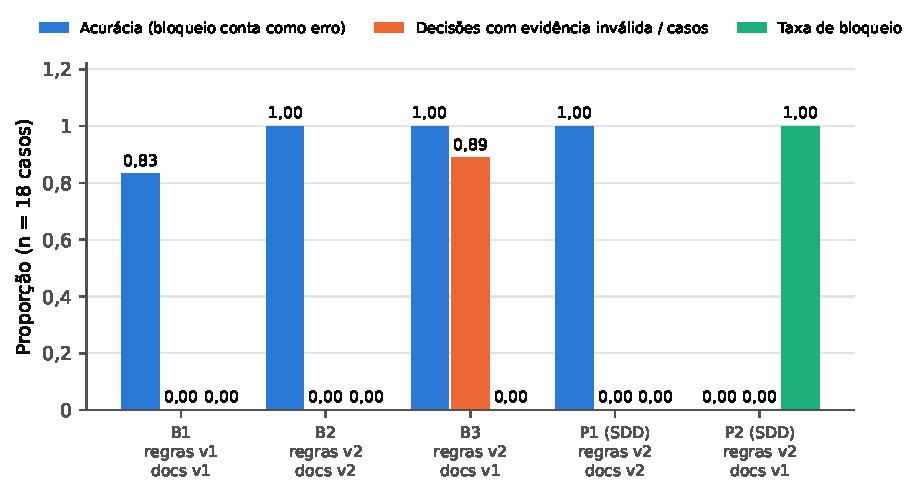
\includegraphics[width=0.95\linewidth]{fig_benchmark_condicoes.pdf}
\caption{Acurácia, evidência inválida e bloqueio nas cinco condições da demonstração.}
\label{fig:benchmark}
\end{figure}

\subsection{Estudo de Mutações}

Partindo do par sincronizado (especificação v2 e documentos v2), doze operadores produzem derivas reais (M01--M12) e seis produzem mudanças benignas (N01--N06), com rótulo de verdade atribuído \textit{a priori} (Tabela~\ref{tab:mutantes}). Cada mutante é validado nos quatro níveis e os 18 casos são executados com guarda. A Figura~\ref{fig:matriz} mostra o resultado mutante a mutante.

\begin{table}[!ht]
\centering
\caption{Operadores de mutação do estudo exploratório.}
\label{tab:mutantes}
\scriptsize
\begin{tabularx}{\linewidth}{l X l X}
\toprule
\textbf{ID} & \textbf{Deriva injetada} & \textbf{ID} & \textbf{Mudança benigna} \\
\midrule
M01 & limiar alterado só na especificação & N01 & reordenação de regras \\
M02 & precedência trocada & N02 & reordenação de requisitos \\
M03 & decisão invertida & N03 & reordenação de documentos \\
M04 & regra removida & N04 & metadados editoriais \\
M05 & requisito removido & N05 & correção de pontuação no texto \\
M06 & requisito sem regra & N06 & evolução completa e sincronizada \\
M07 & justificativa contraditória & & \\
M08 & atualização parcial (um documento antigo) & & \\
M09 & texto editado sem revisão & & \\
M10 & texto invertido com marcas recalculadas & & \\
M11 & limiar alterado com marcas recalculadas & & \\
M12 & base documental v1 inteira & & \\
\bottomrule
\end{tabularx}
\end{table}

\begin{figure}[!ht]
\centering
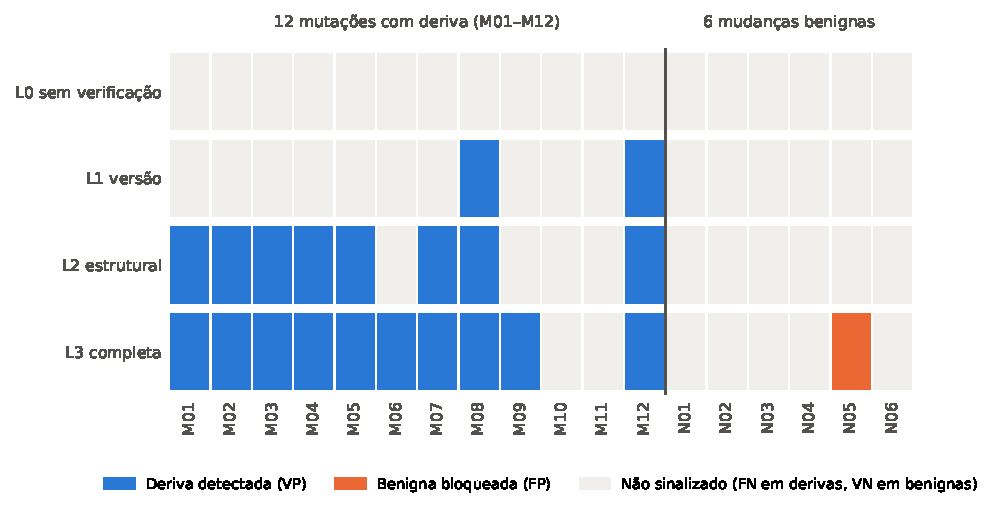
\includegraphics[width=0.95\linewidth]{fig_matriz_deteccao.pdf}
\caption{Detecção por mutante e por nível do validador.}
\label{fig:matriz}
\end{figure}

A Figura~\ref{fig:sensibilidade} agrega os resultados. O versionamento convencional (L1) detecta apenas as duas derivas que mudam a versão declarada (M08 e M12). As marcas de integridade (L2) elevam a sensibilidade para 8/12, sem alarmes falsos. O nível completo (L3) chega a 10/12 ao capturar o requisito sem regra (M06) e a edição de texto sem revisão (M09), mas o \textit{digest} de texto também bloqueia uma correção de pontuação (N05), o único alarme falso observado (precisão de 10/11).

\begin{figure}[!ht]
\centering
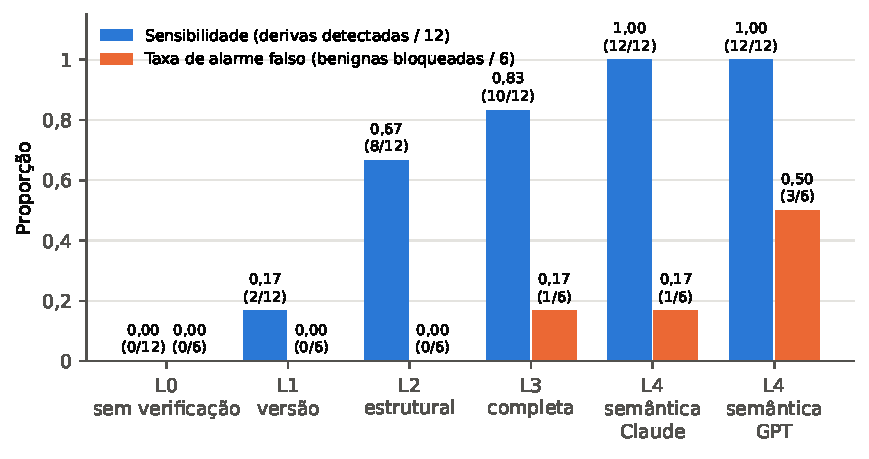
\includegraphics[width=0.9\linewidth]{fig_sensibilidade_niveis.pdf}
\caption{Sensibilidade e taxa de alarme falso por nível do validador.}
\label{fig:sensibilidade}
\end{figure}

A Figura~\ref{fig:impacto} traduz a detecção em efeitos operacionais somados sobre os 18 mutantes. As decisões erradas emitidas caem de 9 (L0 e L1) para 1 (L2 e L3), e as decisões emitidas com evidência divergente caem de 101 para 18. O custo aparece no terceiro painel: em L3, a mudança benigna N05 bloqueia 18 decisões.

\begin{figure}[!ht]
\centering
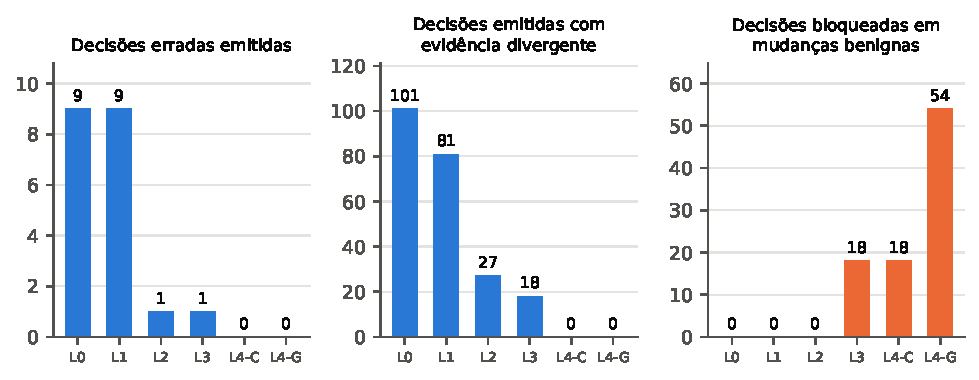
\includegraphics[width=0.95\linewidth]{fig_impacto_operacional.pdf}
\caption{Efeitos operacionais por nível, somados sobre os 18 mutantes.}
\label{fig:impacto}
\end{figure}

\textbf{Limite semântico.} M10 e M11 não são detectados em nenhum nível. Em ambos, o significado é alterado (o texto da política é invertido, ou o limiar muda mantendo o texto antigo) e as marcas de integridade são recalculadas sem revisão do conteúdo. A verificação estrutural é contornada por construção: \textit{fingerprints} e \textit{digests} atestam que os artefatos não mudaram desde a última aprovação, e não que texto e regra dizem a mesma coisa. Esse resultado delimita o alcance da abordagem e motiva a principal extensão do estudo: avaliar se um verificador semântico (LLM como juiz, revisão humana, ou ambos) detecta essa classe de deriva e a que custo.

%%%%%%%%%%%%%%%%%%%%%%%%%%%%%%%%%%%%%%
%%%%%%%%%%%% Seção 6  %%%%%%%%%%%%%%%%
%%%%%%%%%%%%%%%%%%%%%%%%%%%%%%%%%%%%%%
\section{Plano de Pesquisa}
\label{sec6:plano}

\textbf{Questões de pesquisa.} A questão principal é: \textit{em que medida um fluxo orientado por especificações versionadas melhora a detecção de inconsistências e a rastreabilidade de decisões de agentes híbridos ao longo da evolução de políticas de negócio?} Ela se desdobra em quatro questões:
\begin{itemize}[noitemsep, topsep=3pt, leftmargin=1.5em]
  \item \textbf{QP1:} a abordagem aumenta a taxa de detecção de divergências entre especificações, regras e documentos, em comparação com \textit{baselines} sem verificação de coevolução?
  \item \textbf{QP2:} a abordagem reduz decisões justificadas com evidência desatualizada durante atualizações controladas de políticas?
  \item \textbf{QP3:} quais custos adicionais a abordagem introduz (bloqueios, manutenção, latência e revisão humana)?
  \item \textbf{QP4:} em quais condições a verificação estrutural deixa passar divergências semânticas, e qual é o benefício incremental de revisão humana ou de verificação assistida por LLM?
\end{itemize}

As hipóteses são direcionais e orientam a coleta: \textbf{H1}, a verificação SDD tem maior sensibilidade do que o versionamento convencional na detecção de deriva; \textbf{H2}, ela reduz a proporção de decisões emitidas com evidência versionada incorretamente, com bloqueios contabilizados à parte; e \textbf{H3}, ela impõe custos de manutenção e de indisponibilidade mensuráveis e não desprezíveis.

\textbf{Etapas.} O estudo segue as diretrizes de experimentação em Engenharia de Software de \cite{wohlin2012experimentation} e está organizado em quatro etapas:
\begin{enumerate}[noitemsep, topsep=3pt, leftmargin=1.5em]
  \item \textit{Revisão sistemática} \cite{kitchenham2007slr} sobre \textit{policy-as-code}, conformidade de agentes, evolução de bases RAG, rastreabilidade em sistemas com LLM e SDD.
  \item \textit{Corpus de mudanças e operadores de mutação}, com múltiplas políticas e famílias de mudança (exceções, precedência, limiares, documentos conflitantes, inversão semântica com metadados preservados, atualização parcial e requisitos ambíguos), vários mutantes por família e rótulos atribuídos por avaliadores independentes, cegos ao validador.
  \item \textit{Integração com LLMs e condições experimentais}, sob o mesmo modelo, corpus, limite de \textit{tokens}, temperatura e tarefas: B1 (agente RAG sem guardas de regra); B2 (agente RAG com regras determinísticas e validação de saída); B3 (B2 com versionamento convencional); P (B3 com verificação SDD, rastreabilidade e bloqueio); e P+S (P com verificação semântica assistida por LLM). O \textit{baseline} B3 permite atribuir os ganhos à verificação SDD, e não apenas ao versionamento; P+S responde a QP4.
  \item \textit{Análise}, com sensibilidade e precisão dos alertas, acurácia com bloqueios reportados à parte, cobertura, validade da evidência, rastreabilidade e custo (latência p50/p95, \textit{tokens}, esforço de atualização e taxa de revisão humana). Intervalos de confiança serão estimados por \textit{bootstrap} agrupado por cenário \cite{efron1993bootstrap}, e comparações pareadas de acerto binário usarão o teste de McNemar \cite{mcnemar1947}, com correção para comparações múltiplas. O tamanho amostral será definido por estudo piloto e análise de poder, e o protocolo será pré-registrado.
\end{enumerate}

\textbf{Cronograma.} A Figura~\ref{fig:cronograma} apresenta o cronograma previsto para 24 meses. Para doutorado, as etapas 2 a 4 podem ser repetidas em mais domínios e complementadas por estudo de caso em ambiente real \cite{runeson2009casestudy}.

\begin{figure}[!ht]
\centering
\resizebox{0.9\linewidth}{!}{
\begin{ganttchart}[
  hgrid, vgrid={*2{draw=none}, dotted},
  x unit=0.32cm, y unit chart=0.55cm,
  bar/.append style={fill=blue!25, draw=blue!60, line width=0.7pt, rounded corners=1pt},
  milestone/.append style={fill=red!50, draw=red!60},
  bar label font=\small, title label font=\small,
  bar height=0.55
]{1}{24}
  \gantttitle{Trimestres (24 meses)}{24}\\
  \gantttitlelist{1,...,8}{3}\\
  \ganttbar{Disciplinas obrigatórias}{1}{12}\\
  \ganttbar{Revisão sistemática}{1}{6}\\
  \ganttbar{Corpus e operadores de mutação}{5}{10}\\
  \ganttbar{Integração com LLMs e condições}{8}{14}\\
  \ganttmilestone{Qualificação}{12}\\
  \ganttbar{Rotulagem independente e piloto}{11}{14}\\
  \ganttbar{Coleta confirmatória}{15}{18}\\
  \ganttbar{Análise e artigo}{17}{21}\\
  \ganttbar{Redação da dissertação}{18}{24}\\
  \ganttmilestone{Defesa}{24}
\end{ganttchart}}
\caption{Cronograma previsto.}
\label{fig:cronograma}
\end{figure}

%%%%%%%%%%%%%%%%%%%%%%%%%%%%%%%%%%%%%%
%%%%%%%%%%%% Seção 7  %%%%%%%%%%%%%%%%
%%%%%%%%%%%%%%%%%%%%%%%%%%%%%%%%%%%%%%
\section{Ameaças à Validade}
\label{sec7:ameacas}

Em relação à \textit{validade de construto}, \textit{fingerprints} e \textit{digests} verificam estrutura e integridade, não significado, e o oráculo exige revisão independente. Quanto à \textit{validade interna}, um \textit{baseline} simplificado favoreceria a proposta, por isso as condições serão pareadas em funcionalidade e recursos; além disso, mutantes escritos pelo mesmo autor do validador introduzem viés de construção, a ser mitigado com geração sistemática e rotulagem por terceiros. Quanto à \textit{validade externa}, políticas fictícias não representam sistemas regulados reais, e o estudo buscará ao menos um cenário inspirado em documentação pública de um domínio real. Quanto à \textit{validade de conclusão}, casos correlacionados exigem unidade de análise adequada, e o uso de poucos LLMs restringe a generalização. Por fim, do ponto de vista operacional, a política \textit{fail-closed} aumenta bloqueios, cujo custo será medido e reportado.

%%%%%%%%%%%%%%%%%%%%%%%%%%%%%%%%%%%%%%
%%%%%%%%%%%% Seção 8  %%%%%%%%%%%%%%%%
%%%%%%%%%%%%%%%%%%%%%%%%%%%%%%%%%%%%%%
\section{Considerações Finais}
\label{sec8:final}

Este projeto propõe o EvoPolicy-SDD, uma abordagem orientada por especificações para manter verificáveis os vínculos entre requisitos, regras executáveis, documentos de evidência e decisões de agentes de IA ao longo da evolução de políticas de negócio. O protótipo atual mostra, em pequena escala, que as marcas de integridade explicam a maior parte do ganho sobre o versionamento convencional (de 2 para 8 derivas detectadas em 12), que o \textit{digest} de texto amplia a detecção ao custo de bloqueios por mudanças benignas, e que derivas semânticas com marcas recalculadas escapam a qualquer verificação estrutural.

Do ponto de vista científico, o trabalho pretende contribuir na interseção entre Engenharia de Software, rastreabilidade e sistemas baseados em LLMs, com um estudo controlado sobre ganhos, custos e limites da verificação de coevolução. Do ponto de vista prático, pretende oferecer um mecanismo aplicável a equipes que operam agentes sobre políticas que mudam com frequência, sem substituir a revisão humana. Como próximos passos, estão a revisão sistemática, a ampliação do corpus de mudanças e a integração com LLMs reais, incluindo a avaliação da verificação semântica como resposta ao limite identificado.

%%%%%%%%%%%%%%%%%%%%%%%%%%%%%%%%%%%%%%
%%%%%%%% Disponibilidade  %%%%%%%%%%%%
%%%%%%%%%%%%%%%%%%%%%%%%%%%%%%%%%%%%%%
\section*{Disponibilidade dos Artefatos}
{
\small
O protótipo EvoPolicy-SDD v0.1.1 será disponibilizado como material suplementar e em repositório público. Esse material inclui: (i) código-fonte do pacote \code{evopolicy} e sua suíte de 35 testes automatizados; (ii) especificações v1 e v2, bases documentais e os 18 casos sintéticos rotulados; (iii) resultados brutos da demonstração e do estudo de mutações (\code{results/}), incluindo o registro auditável das decisões; e (iv) o \textit{script} que gera as figuras deste texto a partir desses resultados.
}

%%%%%%%%%%%%%%%%%%%%%%%%%%%%
%%%%%%%%% Uso de IA %%%%%%%%
%%%%%%%%%%%%%%%%%%%%%%%%%%%%
\section*{Uso de Inteligência Artificial}
\label{Sec:IA}
{
\small
Em conformidade com o Código de Conduta para Autores da SBC, declara-se que ferramentas de IA foram utilizadas como apoio. O \textit{Claude} (Anthropic) foi utilizado como apoio à implementação do protótipo, à geração das figuras a partir dos resultados e à redação e organização deste texto, sendo o conteúdo científico, a verificação das referências e as conclusões apresentadas de responsabilidade exclusiva do autor.
}

\bibliographystyle{sbc}
\bibliography{references}

\end{document}
